%課題研究レジュメテンプレート ver. 1.0

\documentclass[uplatex]{jsarticle}
\usepackage[top=20mm,bottom=20mm,left=20mm,right=20mm]{geometry}
\usepackage[T1]{fontenc}
\usepackage{txfonts}
\usepackage{wrapfig}
\usepackage[expert,deluxe]{otf}
\usepackage[dvipdfmx,hiresbb]{graphicx}

\makeatletter
  \renewcommand{\section}{%
    \if@slide\clearpage\fi
    \@startsection{section}{1}{\z@}%
    {\Cvs \@plus.5\Cdp \@minus.2\Cdp}% 前アキ
    {.5\Cvs \@plus.3\Cdp}% 後アキ
    %{\normalfont\Large\headfont\raggedright}}
    {\normalfont\raggedright}}

  \renewcommand{\subsection}{\@startsection{subsection}{2}{\z@}%
    {\Cvs \@plus.5\Cdp \@minus.2\Cdp}% 前アキ
    {.5\Cvs \@plus.3\Cdp}% 後アキ
    %{\normalfont\large\headfont}}
    {\normalfont}}

  \renewcommand{\subsubsection}{\@startsection{subsubsection}{3}{\z@}%
    {\Cvs \@plus.5\Cdp \@minus.2\Cdp}%
    {\z@}%
    %{\normalfont\normalsize\headfont}}
    {\normalfont}}
\makeatother
%ここから上を編集する必要はない.





\title{\vspace{-14mm}GitHubにおける開発フローの判別分析}
\author{PMコース 矢吹研究室 1242132 若月 純}
\date{}%日付を入れる必要はない.
\pagestyle{empty}%ページ番号は振らない.
\begin{document}
\maketitle





\section{研究の背景}

ソフトウェア開発では,複数のメンバが同時に開発を行うため,ファイルの最新バージョンが分からなくなる,同一ファイルに対する変更が競合する等の問題が発生する.このような問題を解決するため,バージョン管理システムを用いる.バージョン管理システムとは,変更履歴を管理するシステムのことである\cite{ikeda2014}.

バージョン管理システムを提供するサービスに,GitHubがある.GitHubは,バージョン管理システムに加え,branch,Pull Requestといった開発を補助する機能を提供するサービスである.branchとは,履歴を分岐して記録していくためのものである.branchを用いることにより,同一リポジトリ内で,別々の作業を並行して行うことが出来るようになる.Pull Requestとは,自分のリポジトリから相手のリポジトリへ変更を取り込んでもらうための要求を出す機能である.Pull Requestを用いることにより,変更が追加される前に確認することが出来る.

GitHubを使用する手順を開発フローと呼ぶ.現在わかっている開発フローの数は13個ある.開発フローの例を2つあげる.
GitHub Flowは,作業をするbranchを作成し,完成したら統合する.というような開発フローである.この開発フローはとてもシンプルなため,開発フローを実施するまでの学習コストは抑えられるが,開発規模が大きい場合,Pull Requestがたまりやすく,コードレビューに時間がかかってしまうことがある.
Git Flowは,develop branchから作業用branchを作成する.完成したらPull Requestを行い,develop branchに統合する.リリースができるレベルになったら,リリース用branchを作成し,作業をする.リリース作業が終了するとmasterブランチに統合され,バージョンタグを打ってリリースする.というような開発フローである.branch別にやることが決まっているため管理は容易であるが,複雑すぎるため,Pull Requestを異なったbranchに送ってしまう等の人的ミスが発生する場合がある\cite{otsuka2014}.

このように開発フローは,メリットとデメリットがある.適切でない開発フローを選択すると,デメリットが多く発生する場合がある.このような事態を防ぐために,開発フローをプロジェクトの性質から選択する基準が必要である.しかし,選択する基準は定められていないため,適切な開発フローを選択する基準を明確にすることが必要である.

\section{研究の目的}

GitHubを用いたソフトウェア開発プロジェクトの性質において,適切な開発フローを選択できるようにするための基準を提供する.

\section{プロジェクトマネジメントとの関連}

ソフトウェア開発プロジェクトにおいて,プロジェクトマネージャーは,QCDを達成させるためにスケジュール,コスト,品質コントロールを行う.これらのコントロールを,GitHubを用いた開発フローを導入することで,補助することが出来る.

\section{研究の方法}

本研究は2段階に分かれる.
\begin{enumerate}
\item GitHub上のプロジェクトから,プロジェクトの性質と開発フローを調査する.
\item 調査したデータの分析をする.
\end{enumerate}

プロジェクトの性質は,開発人数,言語,行数を調査する.開発人数と言語は,GitHub上のデータを用いる.

開発フローは,GitHub上のbranch,Pull Requestの特性から求められる.branchにstableが用いられている場合は,Stable Flowである.master branchから記述的な名前のbranchがある場合は,GitHub Flowである.develop branchとrelease branchがある場合は,Git Flowである.バージョンごとにbranchが作られている場合は,LINE Flowである. Pull Request にWIPがある場合は,WIP Flowである.

調査したデータの分析は,決定木分析を行う.決定木分析により,プロジェクトがどのような性質を持つときに,どの開発フローが使われているかを明らかにする.



\section{現在の進捗状況}

\begin{wrapfigure}[14]{r}{9cm}
\vspace*{-\intextsep}
%\includegraphics[width=図の幅,clip]{ファイル名}\label{参照用ラベル}
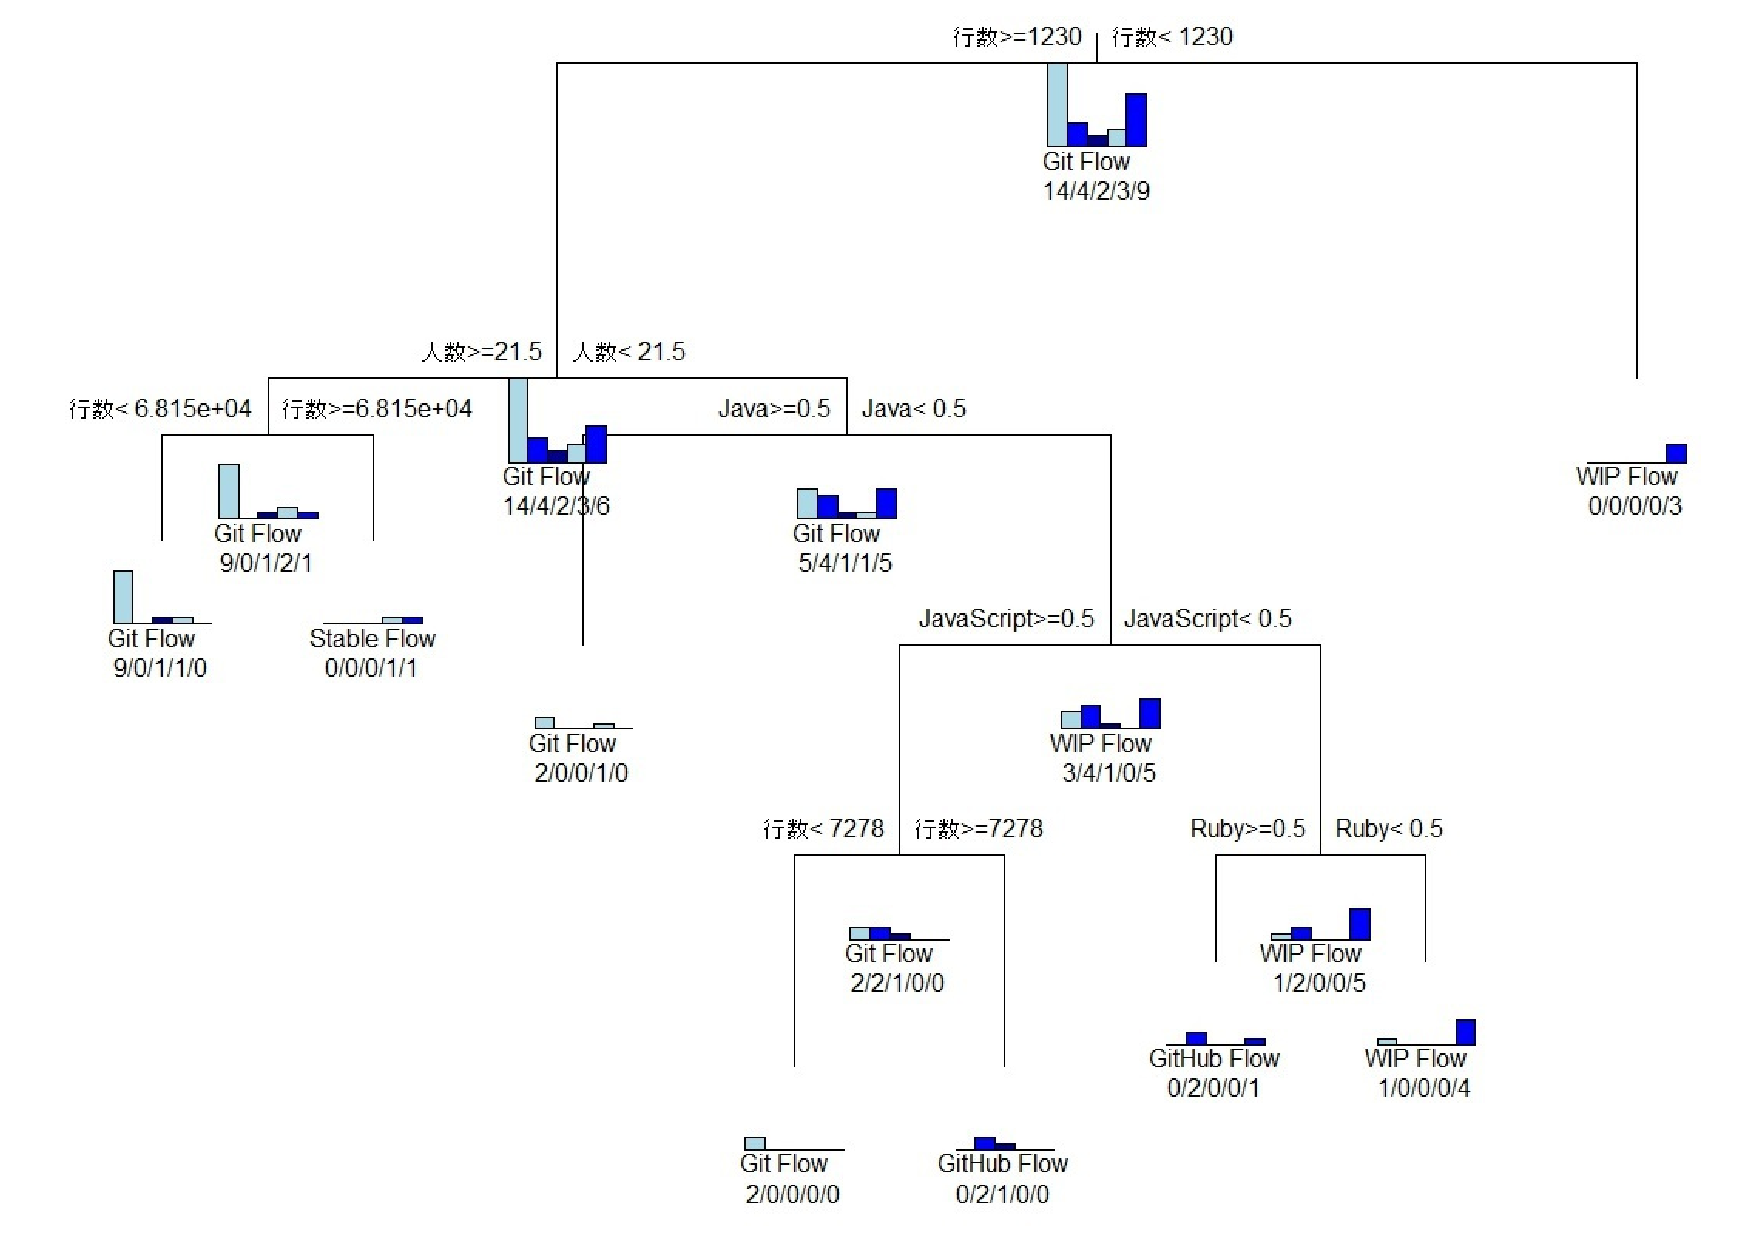
\includegraphics[width=9cm,clip]{images.pdf}
\caption{プロジェクトの性質により選択される開発フローの違い}\label{決定木}
\end{wrapfigure}

GitHub上の32個のプロジェクトから,プロジェクトの性質と開発フローを調査し,決定木分析を行った.

プロジェクトの性質は,開発人数,言語,行数を調査した.開発人数は最少3人,最大156人だった.言語は,Java,JavaScript,Ruby等19種類だった.行数は最小695,最大875841だった.

開発フローは,Git Flow,GitHub Flow,LINE Flow,Stable Flow,WIP Flowの5種類だった.

決定木分析結果は,図1である.分析結果から,プロジェクトの性質により選択される開発フローが明らかにされた.
22人以上の場合,GitHub Flowが使われていないことがわかる.GitHub Flowは,開発人数が多くなると管理が難しくなるためであると考えられる.
また,言語により使われている開発フローに違いがあることがわかる.これは,言語により開発スピードが異なり,管理方法も異なるためであると考えられる.

\section{今後の計画}

現在の開発フローを選択する基準は,人数の場合,21人以下と22人以上で別れている.そのためプロジェクトメンバが5人の場合と15人の場合,同一の開発フローを選んでしまう.しかし,プロジェクトメンバが5人の場合と15人の場合では,プロジェクトの性質は大きく異なり,同一の開発フローを選択するとデメリットが発生する可能性がある.そのような事態を防ぐため,開発フローを選択する基準を,より詳細なプロジェクトの性質で決められるようにする.

データ数が増えれば,より詳細なプロジェクトの性質で開発フローを選択する基準を明確にすることが出来ると仮定し,以下のように研究を進める計画である.

\begin{enumerate}
\item GitHub上のプロジェクトから,プロジェクトの性質と開発フローを調査する.
\item 調査したデータを元に分析を行い,開発フローを選択する基準を明確にする.
\item 論文の執筆を行う.
\end{enumerate}
\bibliographystyle{junsrt}
\bibliography{biblio}%「biblio.bib」というファイルが必要.

\end{document}
